\section{Deep Space Communications}
\label{sec:space}

There are fundamental differences between space-based communication and traditional communication on the earth. Understand the physical limitations of communication in deep space is fundamental at the time of design secure protocols. This section gives a review of the principal components of space-based communication, the evolution of the communication model for space missions and provide a security overview of space-based networks.

The launch of the Sputnik 1 satellite gave origin to the Space Race. Human spaceflights and unmanned robotic space probes were developed to support space exploration missions. A communication system was needed to send commands from a mission control centre and receive information from spacecraft. The original idea was simple: the mission control centre sends a Radio Frequency (RF) signal to a spacecraft, known as telecommand, the spacecraft receives the signal via its antenna and process the telecommand, then the spacecraft replies with telemetry command or science data if necessary. As space missions grew in complexity and distance to the earth, communication systems had to evolve to keep the pace. 

A simplified diagram of a space mission architecture is shown in the figure \ref{fig:space-based-arc}.  


\begin{figure}[ht]
\centering
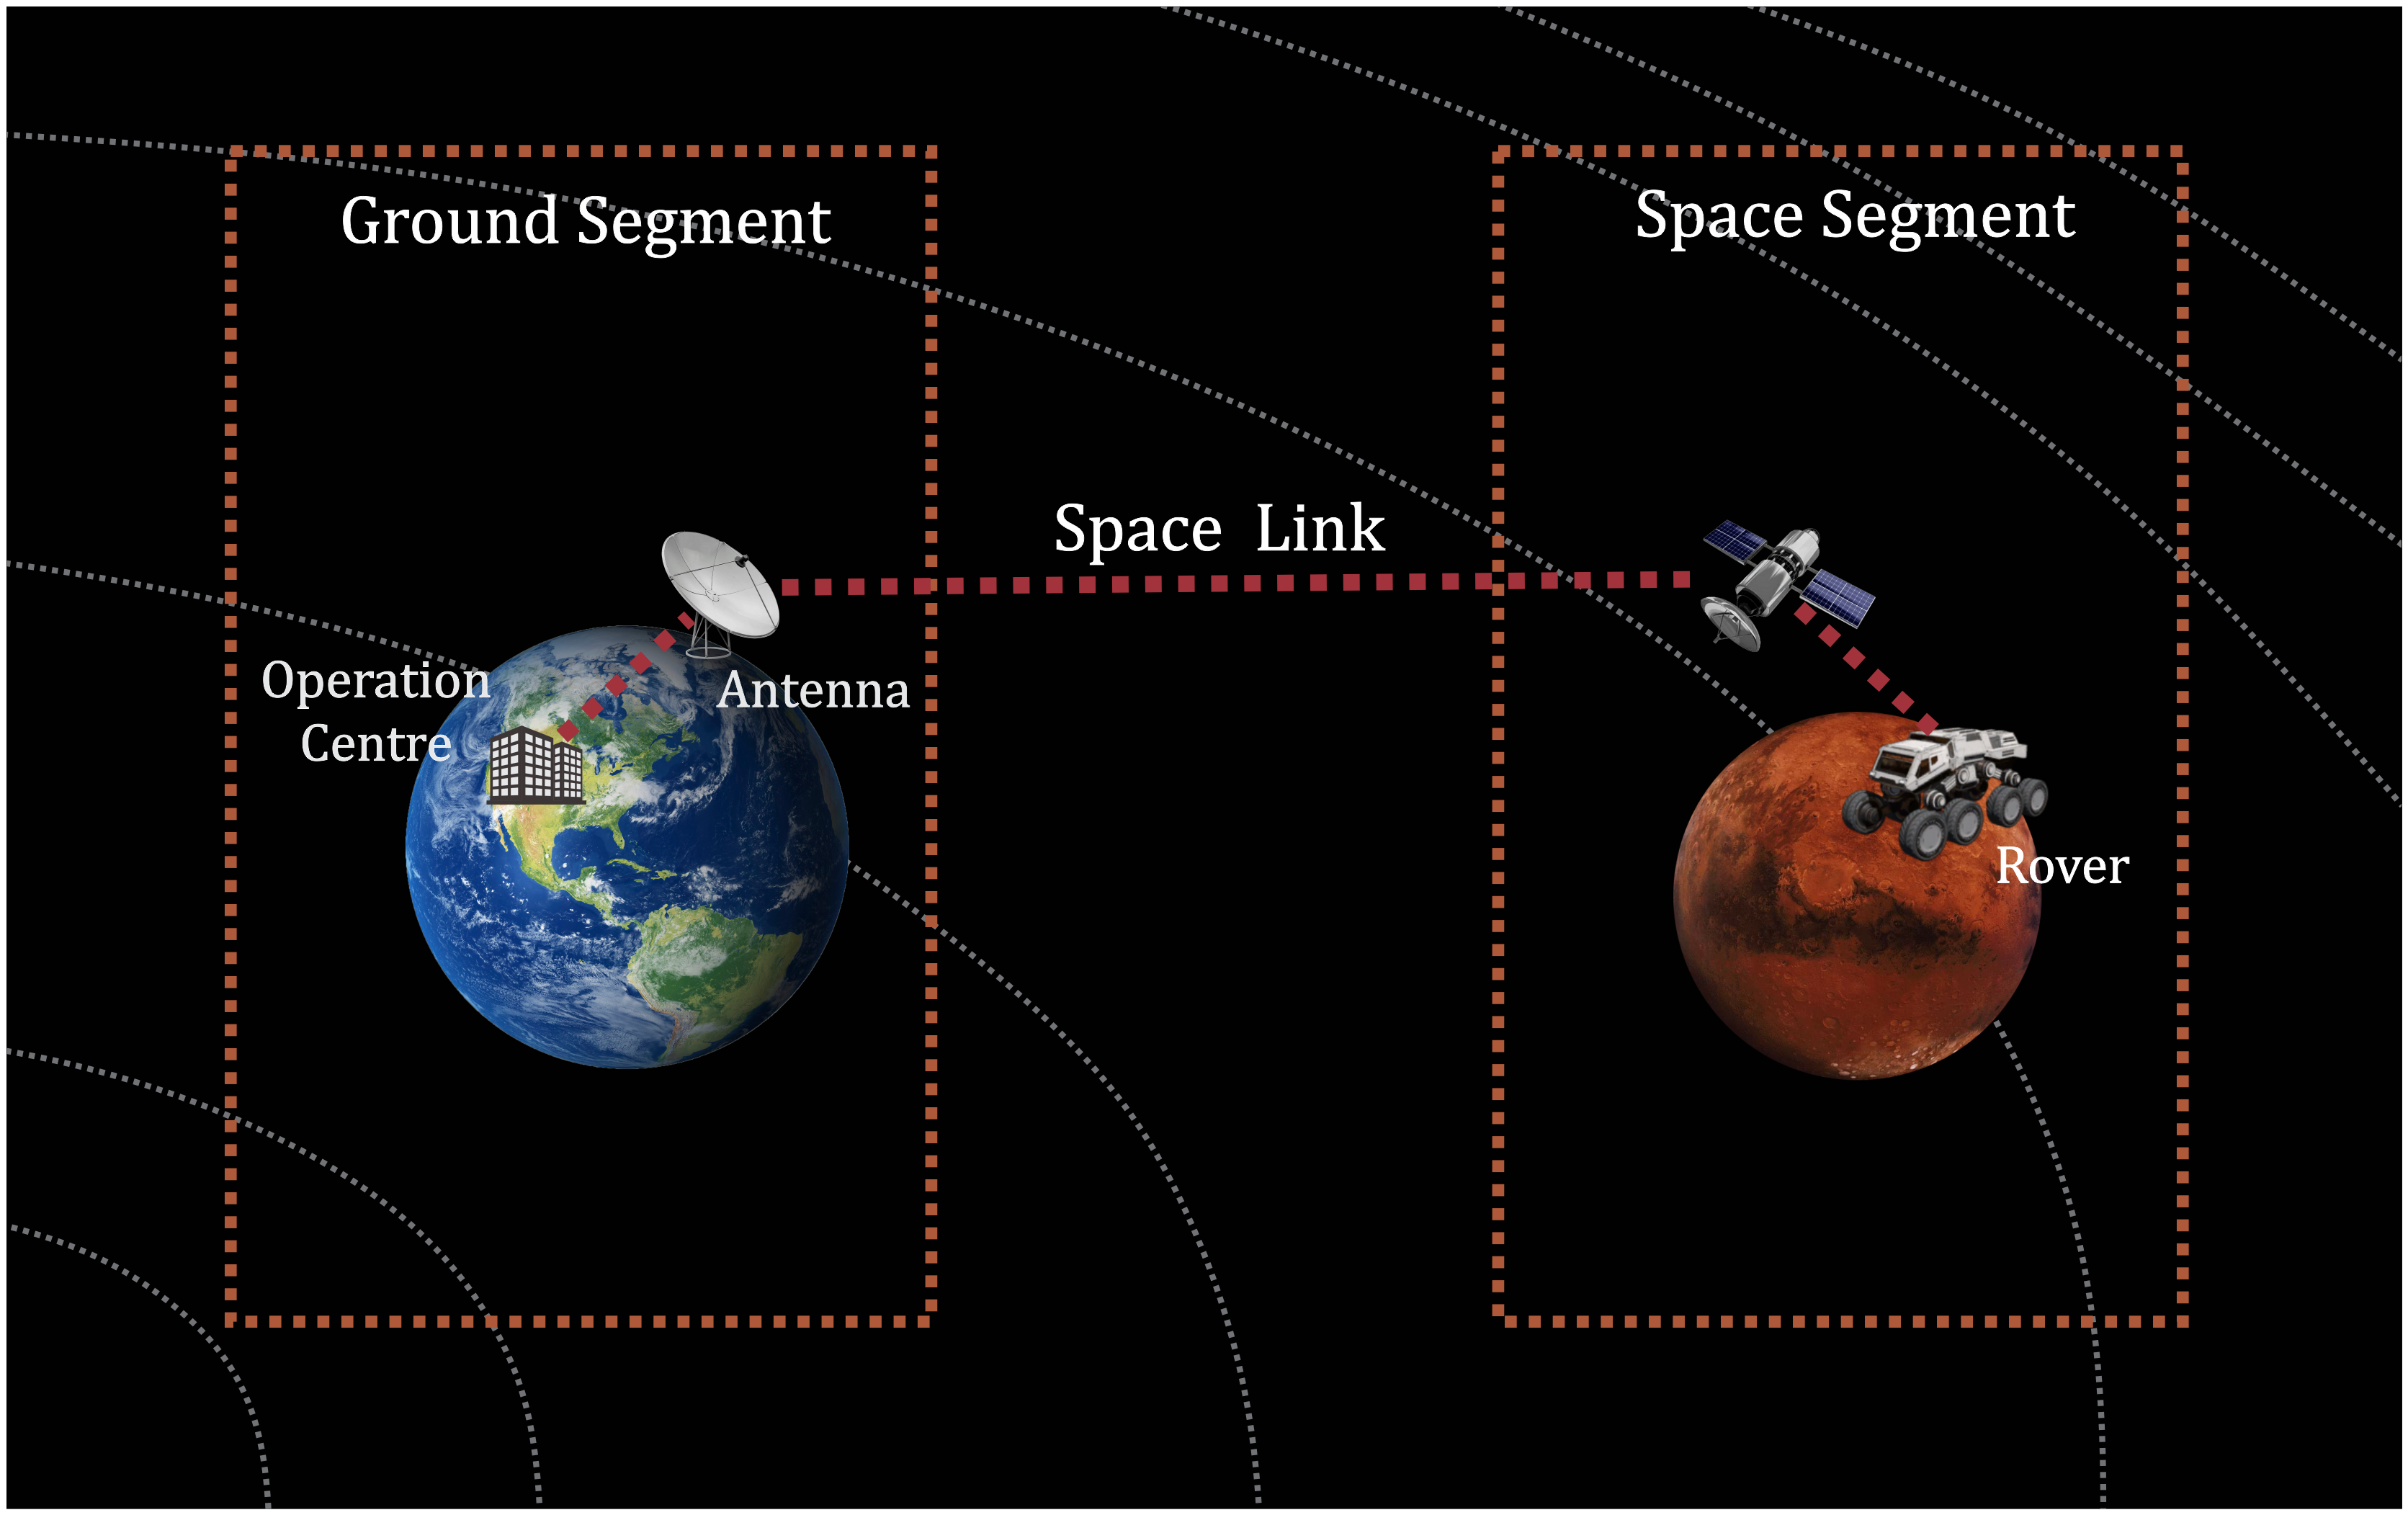
\includegraphics[width=1 \linewidth, height=9.5cm]{images/ground.png} 
\caption{Space-based communication architecture}
\label{fig:space-based-arc}
\end{figure}

In this example, the satellite and the lunar rover form part of the space segment. The space-link segment is the connection between the ground station and the satellite.  The ground station and the mission control centre constitute the ground segment. The mission control centre, sometimes called Operational Control Centre (OCC) has the control of the objects in deep space.

 The most significant differences of space-based communication are the long propagation delay due to the speed of light and the lack of end-to-end connectivity caused by planets motion, resulting in the disruption of connectivity between a mission control centre and space objects. These properties make well-known protocols for terrestrial networks unsuitable for space communications \cite{fall2003delay}.


The distance of an object to the earth determines the type of the communication between spacecraft and ground stations. Near-earth communications present low delay and intermittent connectivity. Satellites in geosynchronous orbit are subject to low delay but continuous connectivity. Earth-Moon communication is a particular case, the round-trip delay is approximately 2.5 seconds, and there is a disruption in the communication due to the motion of the earth and the moon. Deep space missions beyond the moon present the worst case: extremely long propagation delay and disrupted communication. For instance,  a signal from the farthest human-made object in deep space (Voyager 1) takes over 19 hours to reach the Earth. Signals sent by Mars rovers take between 7 and 20 minutes to reach Earth, depending on Earth-Mars relative position. Moreover, a rover has to be in line-of-sight of an orbiter or the Earth to send or receive data, producing disrupted communication. 



There are significant limitations to the current communication model in space missions. Firstly,  the communication between a spacecraft and its mission control centre is mainly point-to-point. Second, each mission operates independently, thus the cooperation is almost nonexistent, although Mars exploration is an exception. An example is bespoke communications protocols; a space mission typically focuses its resources on immediate problems and subsequent mission have to ``reinvent the weel'' \cite{burleigh2003interplanetary}. 

However, over the last years, there is an effort from CCSDS and other bodies like IETF to standardised communication protocols for space missions. Examples include Space Packet Protocol and the Bundle protocol for space communication, both developed by CCSDS.% \cite{standard2010ccsds}. 

Mars exploration motivated the use of orbiters as hop relay nodes between rovers and mission control centre back on Earth. This relay mechanism was the first advance towards a packet-switched network; however, there is no proper inter-networking yet under this configuration. Mars rovers use available orbiters as intermediate hops, but there is no addressing scheme, no classes of data and no proper network layer. These limitations will restrict operations of future missions which will require more communication between space and ground segment \cite{rationale2010requirements}. 


The experience has shown the advantages of multi-hop communication over point-to-point communication. Some of them are: increase in science data return, lower power and hardware requirements for nodes, and more contact opportunities \cite{rationale2010requirements}. Besides, it is predicted that future space mission will operate in an environment of interoperability and cross-support across space agencies. Spacecraft, satellites, rovers and other human-made objects will act as a network of space-based entities as shown in figure XXX.




INSERT FIGURE!!!


\subsection{Security in Space Communications}



Nowadays,  cyber threats apply to all kind of information systems especially the ones administrated by nation-states. Space systems are becoming more interconnected to terrestrial systems.   In this environment, space missions could be the target of malicious attackers.  In the past, only military missions were highly protected, but this is not valid anymore, and all mission requires a level of security \cite{book2006security}.

As the traditional communication model in space missions is point-to-point, data links have been secured using bulk encryption. Although this technique is simple, requires special techniques and hardware to be deployed on both end of the space-ground segment.   Bulk encryption is simple but not scalable, multi-hop communication and interoperability among space agencies exclude bulk encryption for the Interplanetary Internet. Ivancic \cite{ivancic2009security} mention potential problem in the US for international interoperability because The International Traffic in Arms Regulations might have jurisdiction.

The CCSDS present a list of threat sources and types of threats applicable to space missions \cite{book2006security}. The adversaries include terrorist, criminals, foreign intelligence services, computer hackers, and commercial competitors. There are other sources as insiders and structural which require a different attention. Threats could be active or passive. Examples of the first are jamming, unauthorised access, masquerading, Denial of Services, and examples of passive threats are tapping, traffic analysis. The outcome is that threats for space missions should be considered the same way as any other information system.


For many countries, satellites already form part of critical infrastructures like navigation, weather study, and disaster response.  As state before, future missions will require interoperability between space nodes that might be administrated by different agencies. Therefore, space mission planners must consider the implementation of secure communications protocols whether the nodes are in orbit around Earth or exploring remote places in the solar system  \cite{book2006security}.


It is worth to mention that threats could apply to any segment of space missions: space segment, ground segment, space-link segment. Two important points should be noted in the diagram XXX which might affect security.  Firstly, the mission control centre and the ground station are not in the same physical location but requires a secure connection between them. Secondly, the network infrastructure on the earth could belong to one entity and the mission control centre to another.  

An example of the previous idea is the Mars Exploration Mission, which has its mission control in NASA Jet Propulsion Labs but the rovers and orbiters use the Deep Space Network ground stations. This situation suggests that security for the Interplanetary Internet should consider interoperability not only between nodes from different agencies, but it should consider interoperability between the Internet and space segment protocols. 

 %In \cite{book2012architecture}, CCSDS present security requirements for five space mission profile. These profiles are human spaceflight, earth observation, communication, scientific, and navigation. For instance, humans spaceflights present all security requirements but also ``safety-of-life'' and privacy issues. The security of earth observation, navigation, and communications missions vary depending on the information value and the relative position to the earth. Some missions require security for telemetry, telecommands, and payload communication, others only need to secure a subset of those. 
 
 Five space mission profile are presented by CCSDS \cite{book2012architecture}. Each profile demands different security requirements. The profiles are human spaceflight, earth observation, communication, scientific, and navigation. Some missions require security for telemetry, telecommands, and payload communication, others only need to secure a subset of those. Science missions could have spacecraft or robots deployed in remote locations in the solar system. Extra factor should be considered for these missions that could influence security. For instance fault tolerance, the use of intermediate relay nodes and significant mission lifetime.  In multi-organisational missions, payloads and data may belong to different space agencies. Relay satellites and endpoints may be administrated by different agencies as well.
 
 %For instance, humans spaceflights present all security requirements but also ``safety-of-life'' and privacy issues. The security of earth observation, navigation, and communications missions vary depending on the information value and the relative position to the earth. 
 
 %Science missions are more complicated than the previous,  the distance to the earth change requirements dramatically. For interplanetary missions, there are extra factors that should be considered at the time of implementing security, for instance, communication delay, discontinuous communication, fault tolerance, ability to use intermediate nodes (planned and unplanned), significant mission lifetime. The last point to consider is 
 
 %A clear example is optical communications in space, state of the art techniques are not competitive in mass and power performance against radio frequency RF communication, and there are several projects ongoing to meet the performance goals required by mission planners. It remains to see how different profiles could fit in a single key management scheme.
 



\subsection{Key Management for current Missions}

In current space missions, key management complexity is low.  The mission control centre and spacecraft are mainly the entities involve. The mission control centre is responsible for generating, managing and revoking keys. In the context of human-crewed missions, the human intervention in key management operations in deep space is limited. Optionally, the ground station could take part in key management operation if it is working as a security gateway. User facilities may be present if payload data have to be disseminated \cite{book2011space}. 


Typically keys are stored in smart cards and physical protected place. Key generation procedure affects only the ground segment. Master keys are used to generate or exchange new keys of lower hierarchy such as traffic protection keys. In the case that a master key is used as encryption key, all key management operation are conducted before launch. It is possible to use more than one master key in a spacecraft \cite{book2011space}.

Many environmental properties influence a key management solution in space missions. Asymmetric channels and bandwidth restriction, propagation delay, intermittent connectivity, remote locations, limited computational resources and memory. 

Although these limitations imply that symmetric key cryptosystems are more suitable for space missions \cite{book2011space}, future space missions present a different scenario and it is unlikely than symmetric cryptosystems fit the new requirements.

%It is likely to have group key management for multicast within the network.  

